\chapter{Context Of This Research}
\label{chapter:context}

\section{The Scale of The Internet}
\label{section:context scale}

The modern world contains a vast number of electronic devices. The emphasis of this research is on the development of software, so the scope of this research will be limited to devices and systems which include software as a key element. Software is more pervasive, and more complex, than many people think \citep{Kang2015}, though, with software controlled devices ranging from the barely visible and commonplace to multi-million-dollar and planet-wide systems. There are even thousands of computers in space, as they form a key part of every modern spacecraft and artificial satellite \citep{Eickhoff2011}. Increasingly, even small devices, sensors, or appliances include network connectivity and collaborate both with each other and with more traditional computer resources to form the so-called \emph{internet of things}. The internet is already by far the largest and most complex computer system ever built, and every addition makes it even bigger \citep{Belkhir2018}. 

It's hard to get to grips with the scale of the \gls{internet} because so much of it is behind-the-scenes, The most visible aspect of the internet is the \gls{web} (also known as the `www', or just `web'). This may seem relatively simple, because a user can only see at most a few pages at a time, and most people stick to familiar high-profile shopping, social, and informational websites \citep{Similarweb2023}. The web is a \gls{distributed system} consisting of many communicating devices. As originally conceived \citep{Berners-Lee1992} the web was a purely \gls{client-server} system.

Anyone wishing to find some information would use a textual interface or a \gls{web browser} such as the original \emph{NCSA Mosaic} software \citep{Strawn2014} or one of its conceptual descendants such as \emph{Chrome}, \emph{Firefox}, \emph{Edge}, or \emph{Internet Explorer} (which function as the \gls{client}) to request and receive information from one or more data storage machines (known as the \emph{servers}). This is still essentially how the web works today, although extra complexity has been added in the decades since the web's initial design.

Estimates vary as to the `size' of the web and many different approaches have been taken to try and come up with an answer, from random IP-address probing \citep{Xing2003} and undisclosed proprietary algorithms \citep{Murray2000} to lurid websites with unclear data sources\citep{LiveCounter2018}. A slightly more trustworthy estimate is provided by \citet{Worldwidewebsize2018} which at least explains its methodology and data sources \citep{Kunder2008}. This website (at time of writing, 18 March 2024) reports \enquote{at least 5.22 billion pages}. It is important to note, however, that \citet{Worldwidewebsize2018} uses a mechanism based on search engine results and is therefore unable to count unindexed pages such as private (\gls{intranet}) sites, databases, and the so-called `\gls{dark web}'. The real figure is likely to be much larger. A different 2023 survey reported just over a billion websites running on a little over 12 million servers \citep{Netcraft2023} but made no claims about the number of web pages on each site.

As well as being \emph{big}, the web is also very \emph{busy}. There are billions of client devices and many web servers handle millions of requests per day \todo{citation?}. The growth of the \gls{internet of things} is increasing this even more as sensors and other `smart' devices send and receive data without ever involving a human being. Although often described naively as `\gls{the cloud}', the infrastructure of the internet is very physical. Every web request and response passes through a large network of devices including routers, switches, caches, transmitters, receivers, and signal boosters. Each of these contains electronics and the great majority of them also contain software.

A key to understanding the enormous numbers involved is that there is a \emph{lot} of duplication. Many web requests are for the same popular pages, and many pages are very similar to others. The well-known shopping website Amazon.com, for example, currently offers over 350 million products \citep{SellerApp2023}. To make this possible, Amazon uses a set of standard structures for its product pages, with each page differing only in details related to the specific product. The rest of the page is largely the same, with the same branding, layout, headers and footers and so on. Many very high traffic websites need to run multiple servers serving the same website to handle the load, resulting in even more duplication.

Although an increasing amount of the modern web involves some code which runs on the device with the web browser (known as \gls{client-side processing}), the great majority of the work of the web is done on the servers which provide the web browsers with their data. Servers are responsible for listening for requests from browsers using the \gls{http} protocol \citep{rfc2616} or the more secure but otherwise similar \gls{https}, and serving the correct responses. This process can be as simple as generating an error message or locating a stored file and sending the contents in response, or it can involve complex textual and numeric processing, reading multiple files, and collecting data from other servers and databases, before combining the result into a web page or other document ready to return to the client browser.

The huge scale of the internet results in a correspondingly huge consumption of energy. ICT devices and systems require a variety of forms of energy to operate including specific voltages to run micro-circuitry, power to move and spin mechanical parts, and electricity to run cooling fans, illuminate displays, and communicate with other devices. Active web servers are usually located in \gls{datacenter}s, where they have access to the physical security, power, cooling, and connectivity that they need. A single datacenter will often consume the order of tens of megawatts. This would be enough to power thousands, or even tens of thousands, of homes \citep{Law2022}.

Electrical energy consumption contributes to \gls{global warming} in several ways. The most direct is the generation of heat when the electricity is used to perform work. This heat is released into the surrounding environment causing localised warming. Most ICT equipment works best within a relatively narrow temperature range, and if the temperature around the equipment gets too high it needs to be cooled. This in turn requires more electrical energy. While the cooling process may reduce the temperature of the sensitive equipment, it also results in the release of yet more energy as heat into the external environment. Power distribution in a datacenter is usually centralised, which makes it a potential point of failure. Without power, none of the servers in the datacenter would be able to operate. Servers need to run continuously, which means that a datacenter will usually provide additional power systems in case of problems. These additional power systems also consume electricity and release heat, as does the general operation of the datacenter including things such as lighting and security.

The proportion of incoming energy used by infrastructure such as cooling, power conversion and transmission, lighting, security and so on is described using a \gls{PUE} (PUE) metric. The minimum value for PUE is 1.0, which would indicate that the datacenter used no energy for anything except the computing and data storage systems. A 2016 survey reported typical datacenter PUE values in the USA of 2.0 or greater \citep{Shehabi2016}, indicating that more energy was being used by the operation of the datacenter itself than all the IT resources combined. Power transmission from power stations to data centres also loses energy (as heat) along the way, so only a proportion of the power produced by the power station is available at the data centre. As can be see in \autoref{system losses}, less than 20\% of fuel energy typically reaches the servers \citep{Zhao2016}.

\begin{figure}[htbp]
  \centering
  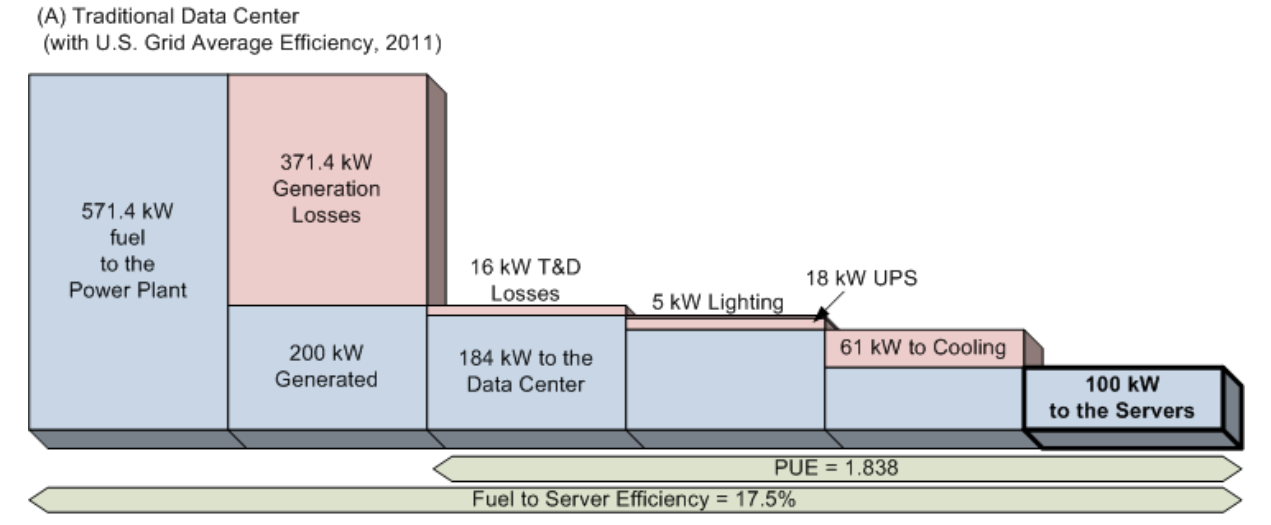
\includegraphics[width=\columnwidth]{Figures/Data-Center-Power.png}
  \caption{Traditional Data Center System Losses (from \protect\citet{Zhao2016})}
  \label{system losses}
\end{figure}

Any power generated by burning fuel, either in a large power station or in a local generator, contributes \gls{greenhouse gasses} such as carbon dioxide to the atmosphere. Greenhouse gasses accumulate in the Earth's atmosphere and contribute to the \gls{greenhouse effect}. These emissions are more serious than localised heating effects, because they are cumulative. If a datacenter were to be shut down immediately, localised heating effects would die down relatively quickly and the local temperature would return to its normal state. The greenhouse gasses, however, will remain in the atmosphere and continue to affect heat retention for much longer, potentially for tens of thousands of years before biological and geological processes absorb or reduce them \citep{Pierrehumbert2019}.

Potential improvements and their effectiveness will be explored in more detail in later chapters, but the key point to note is that all this energy usage and especially all the duplication and losses along the way imply that the field is ripe for change. Small changes in the energy use of key software can have a greatly magnified impact on waste heat and carbon dioxide emissions. Even something as small as a saving of one milliwatt per request on a page which is requested a million times a day, could save a kilowatt per day, every day in server energy usage. Taking into account typical datacenter PUE values and transmission losses, this tiny software change could potentially save over 6kW of power generation and its associated greenhouse gas production. The same logic applies to a page fragment or code component which is used on many different pages. A tiny saving in energy per fragment will result in a much larger overall saving when multiplied by the number of pages which use that component and the number of times those pages are requested.

\section{The History of Computers and Software}
\label{section:context history}

Electronic computing is still a very new field. The first programmable electronic computers generally accepted as such, Colossus and ENIAC, were developed in the 1940s \citep{Campbell-Kelly2023}, still less than 100 years ago. Software, as we might recognise it, came somewhat later. Early computers were distinguished by being large, expensive, often unreliable. and very rare. Software was usually created from scratch for each new need. Initially there were no programming languages or code libraries so each programming task involved designing a solution and laboriously entering it into the computer memory as ones and zeroes. Since then, computers have gained persistent storage, compilers to create the ones and zeroes from readable programs, and a proliferation of \gls{programming language}s. Depending on definitions there are currently between hundreds and thousands of different programming languages \citep{Pigott2020}. The introduction of the web, the browser software to access it, and a slew of data and communication standards, meant that most new computers and operating systems had the ability to participate in a large scale distributed system. With the resources of the web and the communication abilities of the wider internet, collaborating on software development became much easier, leading to the rise of open source, and the spread of free (to use, at least) software libraries and components.

Throughout this process everyone involved has wanted more and more of everything. Faster processing, faster networks carrying more data, bigger and faster storage, bigger screens, more applications with more features. \todo{cite, rewrite, or delete the previous sentence} Software in the 2020s requires a huge amount more resources even to do what is arguably a similar job to that of previous generations. For example, \emph{Wordwise} \citep{Wordwise2023} was a top word processor for the very popular BBC Microcomputer throughout the 1980s. The software was delivered on an 8 kilobyte Read-Only Memory (ROM) chip, and allowed users to write, edit, and print letters and other documents using just 32 kilobytes of memory on a single 8-bit processor running at a clock speed of 2 megahertz. The 2020s equivalent would be something such as \emph{Microsoft Word}, which is usually purchased as part of a subscription to \emph{Microsoft Office}\footnote{\url{https://www.office.com/}} (also known as \emph{Microsoft 365}). Depending on version, this software can take up to around 10 gigabytes of storage space. That's roughly a \emph{million} times more than the 1980s equivalent. Even just the basic Windows 11 operating system can require over 20 gigabytes of storage. A typical 2023 personal computer might have an 8-core processor running at 2 gigahertz. That's roughly \emph{eight thousand} times the processing power of the 1980s word processor.

This explosion in code size is not limited to desktop applications. Web server and \gls{web application} software is far from simple. As of June 2023, the three most popular web server applications were \emph{NginX}, \emph{Apache}, and \emph{Cloudflare} \citep{Netcraft2023}. NginX and Apache are open source software so the details of their code are available online. NginX has roughly 250,000 lines of code \citep{Openhub2023a} while Apache has nearly 1,700,000 lines of code \citep{Openhub2023}. Cloudflare is proprietary software, so details are sparse, but it was apparently based on the NginX codebase, so is probably roughly similar in size.

Of course, people have much higher expectations of modern software, but the facts remain that the single unwavering trend throughout the development of computers and software has been inflation, both of software size and of the resources needed to run it. The sharp increase in the number of `smart' devices joining the internet, the increasing expectations of `\gls{cloud computing}', and the development of various forms of \gls{artificial intelligence} will only push this trend even harder \citep{Falk2023}.

\section{What is Being Done by The Industry}
\label{section:industry}

An obvious method of reducing energy use is to switch off unused computer systems. This technique has even gained a name: `LightSwitchOps' \citep{RedHat2022}. Although simple in concept, this has turned out to be a surprisingly difficult problem, with the main issues being identifying which computer systems are not being used \citep{Lechelt2024}, and gaining access to them to switch them off \citep{Wiggers2023}. Distributed systems comprised of multiple services on multiple physical devices usually run continuously on the basis that a user or another system \emph{might} require access to the service at any time. Actual use of such a system might be rare, so determining whether a particular system should be running requires more than just observing traffic over a short period. A system may actually be obsolete and will never be used again, or it may be largely idle until specific circumstances such as the failure of another system or extra traffic from a busy `Black Friday' sale. Some systems are known to be obsolete but remain active because shutting them down requires access credentials or knowledge which are no longer available. Such unused systems and services have gained the description `\gls{zombie}s' because they remain active and consuming resources even though they should be `dead'. 

On the whole, computing technology has got faster and cheaper every year since its invention. One way which organisations aim to reduce energy usage is to replace old systems with newer, more efficient, ones. Energy reductions can be achieved in two main ways: by replacing a single system with one which is in some sense `better' (usually known as \emph{\gls{upgrading}}), or by replacing several systems by one which is powerful enough to do all their tasks (usually known as \emph{\gls{consolidating}}).

Upgrading has been a popular choice for many years. It is usually relatively simple to implement because it requires no changes to the architecture of the overall system. The new machine can be configured to perform the same roles as the old one, responding to the same addresses and instructions in a way which is indistinguishable to users and other participants. In an ideal situation, the old machine is then switched off, decommissioned and responsibly reused or recycled. This is not always the case, of course, and missing this step of the process is one of the ways in which machines become `\gls{zombie}s'. Upgrading is attractive because it can also provide an increase in capabilities, perhaps storing more data or handling a larger number of requests. However, upgrading does not always reduce energy usage. If the primary purpose of the upgrade is to increase capabilities it is common for the replacement to need at least as much power and cooling as the machine it replaces. This can still be a saving of sorts, if the increase in capabilities were already needed and the alternative was multiple less-efficient machines with a greater total energy requirement than the single new one. This, however, could also be viewed as a form of pre-emptive consolidation.

As well as the operational requirements, energy is also needed to manufacture, transport, and dispose of ICT equipment. Reducing the overall number of computing devices is one way to address rising energy usage. Once zombie machines have been identified and removed, the next step is to find machines which are not being used to their full capacity and consolidate them. Consolidation is a more complex process than simply upgrading old machines. It may require changes to the architecture of the system and the way that elements of distributed systems find and communicate with each other. There may be conflicts with the way the old and new machines are addressed, and so on.

Various technologies have been created to help avoid such problems. The most well established of these is \emph{\gls{virtualisation}}. This is a technique for running several \emph{guest} \gls{virtual machine}s, complete with operating systems, applications, and data on a single (\emph{host}) computer. None of these guest systems is aware of the others. From a software point of view they are completely separate installations. To make this work requires a \emph{hypervisor}. A \gls{hypervisor} is a specific form of \gls{operating system} whose sole job is to manage guest systems and provide them access to the hardware resources without any conflicts. Virtualisation has the advantage that, once the hypervisor is in place, the process of adding a new guest system is usually no more difficult than installing the old system on an upgraded machine of its own. A hypervisor can also provide important management tools such as the ability to take `snapshots' of running systems before making changes, or to migrate a whole virtual machine to a new hardware host without major interruption in service. The main disadvantage of virtualisation is that each guest machine needs a complete software installation including the operating system. This can use a lot of memory and storage resources. Each virtual machine can require many gigabytes of storage and memory, even when the application part of the software is relatively small.

An alternative to \gls{virtualisation} is \emph{\gls{containerisation}}. This has many aspects in common with virtualisation, and provides many of the same benefits in terms of sharing of resources and management tools. In a container system, however, rather than requiring a full installation for each guest machine, several applications can share common facilities such as the operating system and read-only resources. Each containerised application is unaware of the others, and appears to have a whole machine to itself. In most cases the size of a containerised application or system is much smaller than a corresponding virtualised machine image, ideally little larger than the specific resources and code for the application itself. Creating and managing containerised applications is more complex than the equivalent tasks for virtual machines. Each container image must be created using specialist container tools. Although container images are theoretically portable, they can also require specific features of the host system depending on how they were created. Creating, deploying, managing, and updating containerised applications requires very different skills to installing a full system on virtualised or `\gls{bare metal}' hardware.

When upgrading, consolidating, or simply moving a software system to a different machine, the destination does not usually have to be in the same physical location as the original. There are some cases where issues such as physical security or communication latency mean that devices must be situated together, but most distributed system designs are flexible enough that the components can be anywhere with a network connection. This opens up the possibility of \emph{\gls{cloud computing}}. Cloud computing is not a precise or rigidly-defined term but is generally taken to include the leasing of computing and storage resources owned and operated by another organisation. Such resources are usually located in large \gls{datacenter}s where economies of scale can reduce the overheads of running and maintaining a large number of computer systems. Although it is possible to lease whole machines (known as \emph{hosting} or just \emph{leasing}), or in some cases place your own equipment in a shared datacenter (known as \emph{co-location}), cloud computing is mostly achieved using a combination of \gls{virtualisation} and \gls{containerisation}. Full guest images or containerised applications are uploaded to the cloud provider ready to be deployed to appropriate host systems. Most cloud organisations also provide tools to configure virtual networks between these cloud-hosted systems and to make specific ports and services available to the wider internet.

Simply moving a computer system to a different location in a more efficiently run datacenter can have some sustainability benefits, but this must be balanced against the environmental cost of more network traffic when systems are physically separated. The real benefit of cloud computing is in the ability to add or remove additional copies of machines according to demand. In traditional system designs, adding new machines is a slow and costly process involving ordering, installing and setting up new hardware, and often changing the software application as well. Because this process is slow and expensive, such systems are usually designed and built with enough capability to handle the largest expected load. In a cloud system, deploying a new virtual machine or container image is quick and simple enough to be automated and performed only when needed. This allows cloud applications to be set up initially to use just enough resources for normal use. If a service suddenly becomes popular, more machine images can be started to cope with the load, and when that demand drops, some of those extra machines can be stopped again, and their resources returned to the pool for use by other systems. This is commonly known as \emph{\gls{dynamic scaling}}. A system does need to be designed with dynamic scaling in mind, though, to ensure that there are no conflicts when new parts of the application are `spun up' or communication failures when parts are `spun down', and that the operation is generally seamless.

With the increase in awareness of the impact of energy usage, manufacturers have also concentrated on reducing the power consumption of each new generation of technology. A reduction in power consumption is accompanied by the production of less waste heat, which in turn helps to reduce the need for cooling, and thus reduces the power needed for that, too. One of the advantages of designing applications for containerisation is that it becomes relatively easy to rebuild them to take advantage of lower-power hardware as it becomes available. Most cloud providers now offer `greener' hosting options in addition to traditional computer architectures. Sadly, the continual introduction of new and updated technology has its costs, both in financial terms to buy replacement equipment, but also in the energy and resources used in the production of the new equipment and an increase in `e-waste' when the old equipment is discarded. There is a continual trade-off between the impact of continued operation with obsolescent equipment, and the impact of replacing that old equipment with new hardware.

Not all the energy used by the internet is used in server or client machines. A large amount is used in the network itself. The routers, firewalls, transmitters, receivers and signal boosters which make the internet work take energy to operate, and much of this is dependent on the amount of data being transferred. Techniques which reduce the amount of network traffic can also help to reduce energy consumption. In cases where the same data is sent across a network multiple times, such as the content of popular websites or streaming media, local caching can reduce the number of times the data moves across long distances. This also has the advantage of reducing contention for network resources and can potentially provide faster or more reliable access to the content. The increasing demand for machine learning and artificial intelligence can also increase data traffic when large amounts of input data are sent to central servers for processing. The introduction of specialist neural-processing hardware has meant that some of this processing can now be performed at the `edge' of the network, so that only the results of the analysis need to be transferred. 

While these improvements may seem promising, it is against a backdrop of continually increasing demand. Users expect more information, entertainment and commerce to be available online, the rise of remote working places an extra burden on the network, and even many of the attempts to address other aspects of sustainability end up requiring server processing and network traffic. There is no sign of this growth in internet use, or its associated energy usage, slowing down any time soon \citep{Morley2018} \citep{Odlyzko2016}.

In summary, the computer industry is aware of the environmental problems and the energy usage of computer systems, and has made some steps to address these issues. These steps mostly include \gls{virtualisation} and \gls{containerisation}, \gls{cloud computing}, \gls{dynamic scaling} and \gls{upgrading} to `greener' hardware where possible. Despite this, computer and software systems keep growing and the overall energy usage keeps increasing. All of the attempts at improving the sustainability of computer systems discussed in this section have one thing in common. They treat it as a \emph{hardware} problem. Despite all the improvements in capability and efficiency, computer hardware is still essentially fixed. What makes the difference between one system and another is the software. Software was designed for the express purpose of being able to change the behaviour of electronic systems without changing the hardware, but, as will be shown in \autoref{section:literature}, relatively little research has been done into improving the development of software to make it more sustainable.

\section{How Software is Made}
\label{section:context development}

\subsection{Categories of Software}

It is common in the teaching of computing to repeat the notion that there are three types of software: \emph{system software}, \emph{utility software}, and \emph{application software} \citep{FuturelearnTypes} \citep{Gupta2023a} \citep{Various2023} and many more. This distinction was coined during the relatively early days of the development of computing, when most software was created from scratch in isolation to run on standalone computers, and is arguably no longer particularly useful. Modern software is multi-layered and often distributed between multiple machines. Code is shared and re-used at all levels and the boundaries between the three original categories have become blurred and uncertain.

For the purposes of this research it is important to consider the reason for making the software in the first place. For example, software might be created to gain knowledge, or to help people, or even just for the joy of it. This kind of software is generally considered to `non-commercial'. On the other hand, `commercial' software is defined by its association with money, making it, saving it, or both. No two commercial projects are the same, but there is a distinction between software used only within a single organisation and software intended for sale to others. One thing that all commercial software systems and applications have in common is that product features and timelines are driven by business and market analysis rather than personal needs, curiosity, or research funding.

The following sections will consider four rough categories of reason for developing software. These categories are neither strict nor exclusive - examples can easily be found which blur the distinctions, or change over time - but they are potentially useful to examine the way that the reason for creating software affects both the creation process and the end result. the four categories are summarised in \autoref{table:software-categories}.

\begin{table}
\centering
\begin{tabular}{ c | c | c }
  & \textbf{Internal Need} & \textbf{External Need} \\
  \hline
  \textbf{Non-commercial} & \makecell{Open source, personal \\ and hobby software} & \makecell{Academic and \\ research software} \\ 
  \hline
  \textbf{Commercial} & \makecell{Software for use \\ within an organisation} & Software for sale \\
  \hline
\end{tabular}
\caption{Example Software Categories\label{table:software-categories}}
\end{table}

The impact will also be considered of writing software for regulated environments such as banking, medicine, or aviation; the particular challenges of writing software for distributed and web systems; and writing software to be \emph{embedded} in hardware devices.

\subsubsection{Open Source, Personal and Hobby Software}

Personal software projects were once dismissed as just a hobby with no real impact on the wider world. The rise of the open source movement and the increase in acceptance of using open source software in commercial, government, and academic software has changed all that \citep{Midha2011} and now open source software which originated as personal or hobby projects can be found in a huge proportion of applications \citep{Androutsellis-Theotokis2011}. Open source software is almost always made available to users (who are often themselves other developers) for free, although it may have licence restrictions which constrain or prevent commercial use. For the creators, open source software development is often seen as a social good rather than a quick route to riches \citep{Androutsellis-Theotokis2011} \citep{Raymond2010}. An archetypal open source project is created and maintained by a single individual in his or her spare time, which clearly marks it as a hobby rather than a job. Some open source projects do gain enough popularity to attract other developers or enough financial sponsorship to allow the original developer to work on the project full-time, but this is not the norm.

A single person project which has to fit in around work and family life imposes its own set of constraints such as time, cost, and personal motivation. To keep such a project moving, despite the constraints of the situation, and with little or no chance of remuneration, requires a high level of personal motivation, and there are many things which can derail or shutdown development on a project. To help keep motivation, individual open source developers have evolved a wide range of techniques, many of which ignore the wider context of the project and potential alternative solutions in favour of `scratching your own itch' \citep{Raymond1999} \citep{Raymond2010}. This, in turn, has led to a profusion of open source solutions to common developer problems.

The wide variety of open source options can be a good thing. If a component you are trying to use does not entirely suit your needs, then there are usually many more to choose from \citep{Raymond2010}. Often, though, the sheer quantity of options can be overwhelming. As an example, a naive search for a `template engine' at the GitHub open source code repository returned over 12,000 results \citep{GitHub2022}. Template engines will be explored in more depth in \autoref{chapter:performance} and \autoref{chapter:comp energy}. Open source software also varies widely in quality, which can have a major impact on the selection process. Evaluation of open source component quality will also be explored in \autoref{chapter:performance}.

\subsubsection{Academic and Research Software}

Academic readers will likely be familiar with academic software development. Software produced in an academic context is usually very different to that produced by independent open source developers, and also very different to that produced in a commercial context. As a broad generalisation, academic software is usually produced for one of two purposes: for teaching and learning or for research. Sometimes, of course, software produced in an academic context may find its way into public open source projects or into commercial products, but this is not its original intention.

Academic software produced for teaching and learning needs to be short, often short enough to fit on a presentation slide, and it needs to clearly express its learning points. In many cases such teaching software serves no other purpose, and does not need to be complete or even to work. Software produced for teaching is often only made available to enrolled students, and software written by students for assessment is usually kept private to avoid claims of plagiarism, so such academic software is not easy to find and re-use in another project. Software produced for teaching and learning will therefore be excluded from further discussion.

Academic software produced for research is not commonly subject to the length and pedagogical clarity constraints of software produced for teaching and learning. In common with commercial projects, such research software is often developed under a deadline and a budget but still needs to achieve some kind of objective. The main difference is that the objective is research rather than profit. A more subtle difference, though, is that research software is often developed by people with plenty of knowledge of the research area, but not necessarily a lot of experience of software development, In this sense it can have more in common with personal software projects on which the developer is learning at the same time. Similarly, academic software is often developed by individuals or very small teams rather than the larger project teams common on commercial projects.

\subsubsection{Software for Sale}

Some commercial software is intended for packaging and sale to end-users for installation on their own machines. Colloquially known as `shrink-wrap' software, this was the dominant form of software delivery from the 1980s until the early 2000s. In recent years there has been a decline in this form of software, as it is replaced by online applications and `software as a service' \citep{Fan2009}. In order to be successful, software for sale must meet market expectations of quality in terns of functionality, reliability, and usability \citep{Khoshgoftaar2001}. Software which falls short in any of these areas risks loss of sales, or may require more expensive marketing, and may not cover the cost of development.

Shrink-wrap software requires a development process which can deliver distinct versions with marketable features while minimising the burden of end-user support. This kind of software was traditionally sold in the form of physical media such as floppy discs, CD-ROM or DVD discs, or USB storage devices. These typically require the design and manufacture of packaging such as cardboard boxes and CD cases in addition to the media themselves. Such products cost money to manufacture and distribute as well as taking up space in warehouses and retailers. Producing all these physical artefacts for each new product or new release of an existing product is complex and expensive, and can lose a lot of money if sales don't match up to expectations. With the rise of the web, it has become feasible to deliver shrink-wrap software electronically, which can reduce some of the production and delivery costs. Regardless of delivery model, this form of software still relies on the production and marketing of distinct versions with enough features to attract potential customers. Such software requires extensive testing and documentation to minimise problems and customer misunderstandings.

With the growth of the internet and the web, many commercial software applications now exist and operate online. The exact nature of this operation varies, but can include browser-based web applications such as \emph{Gmail}\footnote{\url{https://www.google.com/intl/en_uk/gmail/about/}}, public online services accessed primarily through an Application Programming Interface (API) such as \emph{Amazon Web Services}\footnote{\url{https://aws.amazon.com/}}, and client-server applications which include a custom user interface and access a `back end' server through a remote API. Some applications include a mixture of these approaches, such as \emph{Microsoft Office}\footnote{\url{https://www.office.com/}}, also known as \emph{Microsoft 365}, which includes both a web browser interface and installable local applications or \emph{GitHub}\footnote{\url{https://github.com/}} which includes a web interface, a local application and an online API.

On the whole, the cost of releasing updates to such systems is much less than that for shrink-wrap software, which allows developers to make (or revert) changes without the heavy burden of exhaustive testing and re-documentation, even though this may result in errors. This attitude has been phrased as \enquote{Move Fast and Break Things} \citep{Taplin2018}. While the speed and cost of deployment is much lower for these applications, that has been traded for the increased cost and complexity of \emph{running} the applications. With shrink-wrap software the cost of a computer to run the software and the resources to operate it are borne by the user. With internet applications a large part of the cost and resources to run the software is borne by the manufacturer, who has become the \emph{de facto} operator of the system. More customers may imply more income, but also more operational expenses. 

Shrink-wrap software can be relatively simple, as it typically only needs to cater for a single user at a time on a single machine. Each user has their own distinct installation with no impact on any of the others. Most online applications have to cater for large numbers of users, often concurrently, and yet still maintain usable performance and responsiveness. This dramatically increases the complexity of the systems, and many online applications need multiple separate computers running together to keep up with the demand, and developers are tasked with constructing an application which can work effectively and reliably in this context.

\subsubsection{Custom Software for Use Within an Organisation}

Some commercial software is not built for sale, but for internal use within the organisation to assist in other business functions. An example might be a job scheduling tool for service engineers such as \emph{Work Manager} developed by British Telecom \citep{Garwood1997}. Such software contributes indirectly to the success of the organisation by improving service and decreasing costs rather than directly providing revenue. Such software may be developed and maintained using an internal software development team, if one exists, or it may be contracted out to software development specialists, but the essence is that it is the current needs of the organisation which determine features and timescales.

Unlike the development of software for sale, which is essentially speculative, the developers of software for use within an organisation have direct access to the people and processes involved. This can be a positive factor, in that there is usually no need for lengthy market research, focus groups, or trial releases, but it can also be negative. The developers of internal software are subject to all the social forces and `internal politics' of the organisation. This can result in conflicting requirements from different departments, for example, or staff reluctance to adopt a new system.

Internal software projects can vary widely in size, complexity and cost, but all have in common that they are considered as a business expense to be minimised rather than a source of income to be maximised.

\subsubsection{Regulated Software}

Software developments are not above the law, so there will always be legal as well as practical limits on what can be done. In some situations, however, the person or organisation developing the software is constrained by regulations specific to the kind of software being developed and the intended uses. The specific regulatory requirements vary with, for example, financial services oversight imposing very different constraints to those on medical equipment development. In such situations, the consequences of a `bug' could be very serious, and even potentially fatal, so as much as possible is done to eliminate such problems before the system is made available for use. Software development which is regulated in this way commonly involves more checks during development, lengthier testing before release, a lot more documentation, and generally slower release cycle. It could be considered as the opposite of `move fast and break things'.

\subsubsection{Distributed and Web software}

Any system which consists of multiple items of software running on more than one physical or virtual machine is known as a \emph{distributed} system. The web as a whole is a distributed system, but so are many smaller ones. Developing software for distributed systems has its own challenges, particularly when a system is large or has specialist hardware or software requirements and cannot easily be exercised by a single developer. In such situations, parts of the system must be developed and tested, as far as is possible, in isolation. Combining all the individual parts and ensuring that they work together is the task of \emph{integration}. Depending on the circumstances, this might be a manual process, or it might be automated, but in either case the effect is to delay feedback to software developers about whether any changes they have implemented have made the overall system better or worse. However, attempts have been made to apply software development tools and approaches to improve the management of distributed systems under the umbrella term \emph{DevOps} \citep{Jabbari2016}.

\subsubsection{Embedded Software}

Some software is not intended to run on generic computing platforms, but to interact with specialist hardware. Software which is developed as an integral part of a physical product is known as \emph{embedded} software. Every embedded software project is different but such software commonly operates at a very low level, often without any kind of operating system, and often on very resource-constrained devices. Simple processors and limited available memory are typical in embedded projects, as is the need to write software on one machine and `cross-compile' for deployment to the target device. In some cases, the software is developed at the same time as the hardware and developers do not have access to a real device on which to test the software. These constraints can make developing such software a complex process which requires detailed knowledge of the hardware design and a different approach to testing as well as to finding and fixing problems.

\subsubsection{Software Categories Conclusions}

As a final point, it is important to note that things can change. A software product can migrate between these groups as it develops and matures, which will necessarily affect the software development context and processes needed to work with it. As an example, the \emph{Work Manager} scheduling software mentioned above started life as a standalone academic research project \citep{Lesaint2003}, developed into a distributed system and became a key internal product \citep{Garwood1997}, and was then `spun out' as a commercial online service \citep{Trimble2006}.

\subsection{Other Forces affecting software development}

Software development is not usually done in isolation. Developers produce software systems in the context of existing software and hardware choices and subject to conflicting forces.

\subsubsection{Requirements and Expectations}

An obvious force on development is the presence of `requirements' and the expectation from stakeholders that these requirements will be met. The classic software life cycle usually presumes the presence of customers and requirements, often decided before the design and programming phase of the product begins. While requirements are often specified in such situations, there is also a considerable amount of software development which happens without explicit requirements in the traditional sense. Personal and hobby projects rarely have requirements beyond \enquote{scratching the itch} \citep{Raymond2010} of a particular software developer or small team, and research software is often more exploratory in nature and defined by its results rather than its specification. Software developed using one of the many agile processes \citep{Hoda2017} usually has some form of requirements, although these requirements and priorities are decided during the development process and subject to change rather than established before development starts.

In situations where requirements are present they can have varying degrees of rigidity, from precise specifications which must be followed exactly to loose guidance subject to interpretation. In all such cases, however, the presence of requirements, and the accompanying expectations of customers and other stakeholders exert a force on the software to conform to the requirements and to avoid choices which might prevent those requirements being met. Requirements are generally established using a process of \emph{elicitation}, used to determine the wants and needs of stakeholders. Sustainability requirements have a different character to functional requirements and are treated differently by different disciplines \citep{Venters2017a}. For the purpose of this research, maximising sustainability and minimising environmental impact are considered as implicit requirements as recommended by the Green Software Foundation \citep{GreenSoftwareFioundation2024}.

\subsubsection{Timescales}

Along with the pressure of requirements comes the pressure of timescales. These come in many forms from single hard deadlines to a sequence of deliverables or progress demonstrations with negotiable dates. The pressure of timescales can be more subtle and insidious than that of requirements, as it encourages the making of quick decisions and provides an obvious penalty to taking too long to research or come to a conclusion. This in turn can lead to choices being made without enough information, an outcome which is especially likely in situations where that information is both slow and expensive to obtain.

\subsubsection{Development Costs}

Cost is an issue in almost all software development projects, with the main exception being personal hobby projects which are usually limited more by time than money. Just as with timescales, the pressure to keep development costs low can also act to encourage quick (and cheap) decision-making, although a more thorough investigation is sometimes possible if the predicted cost of an incorrect decision outweighs the estimated cost of the research.

\subsubsection{Available Skills}

The knowledge and experience of team members affects the decisions made during design and development of a software system, both in terms of implementing requirements directly, and in terms of selecting third-party components and tools to use. Lack of experience among the team can also lead to decisions which negatively impact cost or timescales, and in turn increase the pressure to make decisions quickly and cheaply \citep{Jiang2007a}.

\subsubsection{Ethics}

Depending on the nature of the application or system being developed, ethical issues may have a different impact on the choices being made during the development process. Ethics in computer science is largely concerned with the uses or impact of \emph{what} is produced rather than \emph{how} it is produced \citep{Alidoosti2022}. For example, software to control medical equipment or voting machines \citep{Fleischman2010} might be subject to more ethical scrutiny than a calculator or a solitaire game. Individual software developers are not always involved in the decisions about how a software product will be used, particularly if the software they are working on is only a component or library which might be used by other, possibly unknown, applications. In such cases the ethical responsibility rests with the industry as a whole.

\subsubsection{The Dilemma of Sustainability}

While all the pressures mentioned above are well understood and often discussed in the context of software design and development, the dimension of sustainability is much less frequently acknowledged \todo{citation}. Commercial software mostly exists in a money-focused world where income is balanced against outgoings. If the environmental impact of a system is considered it is usually through the lens of cost - the cost of energy, the cost of adding or replacing hardware, the cost of infrastructure, and so on. Unfortunately, cost is a poor proxy for sustainability impact \citep{Barbier1990} and is confused even more by techniques such as offsetting and `carbon credits'.

The issue of sustainability is a dilemma because, while the corporate forces affecting decisions largely overlook sustainability, that does not imply that the individual people involved in making and implementing decisions are oblivious or insensitive. The same person who might act to reduce waste and greenhouse gas emissions at home, or publicly fight for gender equality and social justice, can find themself in a position at work where sustainability is often sidelined or overshadowed by other factors which are more easily mapped to financial gain or loss.

\subsection{Software Development Roles}
\label{section:software development roles}

Irrespective of the situation in which the software is developed, there are many different roles required to make a success of a software product. In personal products and single project products all or most of these roles will be filled by the same person. In larger teams or organisations these roles may be spread out with one or more people filling each role. Software Engineering theory points out that simply adding more people to a project will not usually make it any faster or more efficient \citep{Brooks1995}, but simply reducing the number of people will not always be advantageous either. Taking on too many roles can lead to conflicting priorities, time wasted switching between contexts, and a lack of time for the deep thinking  required to solve complex problems \citep{Newport2016}.

As the broad field of computing has developed, the names and expectations of the roles in software development have changed, evolved and blurred, but a few representative examples are listed in \autoref{table:roles}:

\begin{table}[htbp]
\begin{tabular}{p{2.5cm} | p{10cm}}
\textbf{Role} & \textbf{Responsibilities} \\
\hline
Customer & The person or organisation who sponsors a product or project, or a client representative such as a \emph{Product Owner}. Arbitrates on choices and makes decisions that affect the overall suitability of the product or project. \\
\hline
User & A person who will use the product. Not often involved in software decisions \\
\hline
Project Manager & Ensures that a project completes on time and on budget and meets its aims. Prioritises Requirements. \\
\hline
Architect & Makes technical choices which determine the direction of a product. Divides large systems into smaller subsystems and selects infrastructure such as operating systems, databases and cloud platforms. \\
\hline
Designer & May involve high-level decision-making similar to an architect, or other areas not directly related to software, such as graphical design and user experience design. \\
\hline
Developer & Creates, updates, and fixes the software parts of a project. May also do testing, configuration management, and deployment in some contexts. \\
\hline
Tester & Ensures that the system works as intended. May test manually by using a system like a real user, or create and run automated tests. \\
\hline
Configuration Manager & Builds and deploys complex or distributed systems. Ensures that each release contains correct and compatible versions of all components and services. \\
\hline
Operation & Ensures that the server-side parts of the application are available and functioning correctly. Also involves monitoring availability and managing responsiveness as well as backups and resilience, attack prevention and mitigation, and other cybersecurity functions. \\
\hline
Documentation & Produces and updates documentation, tutorials, usage examples etc. \\
\hline
Support & Responds to questions from clients and users, either answering them directly or passing them on to other roles. \\
\hline
\end{tabular}
\caption{Software Development Roles\label{table:roles}}
\end{table}

\subsection{Example Combinations of Roles}

Although all the roles listed in \autoref{table:roles} have their own responsibilities, they are often combined, and the way that they are grouped together can be indicative of the assumptions and structure of the organisation or project.

\subsubsection{The One-Person Team}
The stereotypical grouping of roles for a small personal or open source project is for one person to do everything in the list above, as well as other organisational functions such as publicity and marketing. This can be a lot to take on, and some roles naturally have greater or lesser priority. Typically, in a one-person team the emphasis is on the architecture, design, and programming roles, with product owner and testing roles usually running second. Sadly this means that build, operation, documentation and support often suffer. If the software is released as open source and becomes popular enough, a community of users or co-developers may emerge and provide some peer support and documentation.

Many of the components which are evaluated in later chapters are the product of one-person teams and this can particularly be seen in the lack of support and documentation.

\subsubsection{The Business Startup Team}
Exemplified by the \enquote{Move Fast and Break Things} attitude \citep{Taplin2018}, many business startups focus strongly on the commercial aspects of a product in order to bring in revenue before things are fully ready. Product owner, designer and architect roles have priority, with documentation and support attempting to make up for the lack of emphasis on programming, testing, configuration management and operation. Often these low-priority roles will be subcontracted, sometimes to just one person.

\subsubsection{The Legacy Software Team}
Once a software product evolves beyond the capability of smaller teams, it is common for the team to grow and for people in the team to take on progressively more specialised roles and responsibility for ever more specific niches. This runs the risk of communication issues as discussed in \citet{Brooks1995}. When developers no longer work closely with their colleagues, the fast-and-loose approach taken by one-person teams and startups becomes increasingly dangerous. A typical response to this is to increase the strictness of the development process, which in turn places a lot more emphasis on testing, build, and configuration management roles, often also accompanied by a growth in the need for documentation and support.

An alternative response to increasing product and team complexity is to make use of a light-weight process which is, however, more formally defined than the ad-hoc approach of a startup team. There are a range of such processes, including SCRUM \citep{Schwaber1997} and Extreme Programming \citep{Beck2000}, which are commonly included under the umbrella term `Agile'. An agile process is characterised by its priorities, for example \enquote{Working software over comprehensive documentation}, as enumerated in the `Agile Manifesto' \citep{Beck2001}:

\subsection{Developer Choices}
\label{subsection:developer choices}

A typical software development role involves a range of responsibilities such as understanding the domain, the problem to be solved, and the constraints on possible solutions; architecture; design; selection of libraries or other components; testing; documentation; planning, communicating with team members and many others. All these responsibilities involve making decisions which can affect the costs and resource usage of the eventual system. The choice between making a new software component and adapting or re-using one which has already been made, for example, is understood to have an effect on duration and cost of development \citep{Gacek2002}. However, such choices also potentially impact other factors such as long-term running costs, power usage, cooling and maintenance needs of the system. Research suggests that these factors are often obscured by the importance placed on `up front' development costs and time to market \citep{Petro2017}, and this is backed up by personal experience.

Evans Data Corporation estimated that in 2017 there were 22 million software developers worldwide, a number that was due to rise to 26 million by 2022 \citep{EvansDataCorporation2018}. All these software developers have different skills, experiences, attitudes and preferences. Software, and the development of software, can be very complex. There are as many ways to develop software as there are individual developers, and even individual developers will vary what they do and how they do it depending on factors such as project requirements, team culture and prior experience.

The software development process can be viewed as a sequence of choices which affect the final software product. Some choices are large and set the scene for many others. Some choices are individual and self-contained. This section explores some of the areas in which such choices are made.

\subsubsection{Solution Architecture}

In most software projects, the biggest and most important decisions are usually in the architecture of the solution. This includes choices such as whether to build software which runs on a client system, a central server, or distributed between multiple participating services, how to deal with the expected number of users and quantity of data, where to store information and how to access it, and so on. Like so many things in software development, there is no clear and universally accepted definition of what constitutes an architectural decision rather than one of the many other kinds of decisions. On the whole, if a decision affects the overall structure of the software system and would have a major impact on the code if it were changed, it is usually considered as an architectural decision.

\subsubsection{Programming Languages and Tools}

There is a class of decisions, however, which sits somewhere between architect and developer responsibilities and can cause demarcation problems among teams - the choice of programming languages and other development tools. Such decisions do not directly affect the structure and capabilities of the final software system, so it could be argued that they fall outside the remit of architecture \citep{Mills1985}. On the other hand, they are major decisions which are not easy to change once a large amount of development work has been done, so it could be argued that they need to be included in the key architectural decisions made at the start of a project. \citep{Spinellis2006}

In some cases it is possible for an architectural decision to be made which pushes the decisions on tools and programming languages `down' to smaller development teams, each responsible for different parts of the overall system. One technique to enable this is \emph{microservices}, in which the architecture of a system is defined as a collection of collaborating smaller subsystems, each of which communicates only though a predefined interface, allowing development teams freedom to use whatever development tools, languages, and approaches are most suitable for that subsystem \citep{Chen2022}.

\subsubsection{Testing}

Software testing is itself a complex field \citep{Whittaker2000} which is largely beyond the scope of this research, but there are some key choices which software developers always need to make during the development process. The first of these key choices is \emph{when} to test the code. A software developer continually faces choices about whether to test their code before, during, or after development. Even having decided \emph{when} to test, there are also choices about \emph{what} to test. At one end of the scale it's probably too much work for too little return to try and test every line of code individually, but at the other end waiting for a whole system to be created before attempting to test any of it makes finding which part of the code caused an error much harder \citep{Singh2012}. Some testing approaches such as Test-Driven Development \citep{Beck2022} have been observed to affect the structure and quality of the code itself \citep{George2004}.

\subsubsection{`Green field' or Code Reuse?}

The way programming is often taught, the next step after the requirements and architectural decisions is to decide on the algorithms and data structures which will form the final software, and then start creating code. While there is eventually an aspect of this kind of programming, it is hardly ever as simple as that \citep{Cusumano1995}. Real software rarely starts from a blank page but has to fit in with other parts of the system and conform to the choices which have already been made \citep{Spinellis2006}. Even so-called `green field' software development - creating something new rather than adding features or fixes to existing systems - almost always involves finding existing code or libraries which do part or all of the job \citep{Bjarnason2023} \citep{Sametinger1997}.

Existing code can be used in one of two ways: \emph{White Box} (also known as \emph{Copy and Paste}) - in which the external code is added directly into the project and then modified to suit, and \emph{Black Box} - in which the external code is added to the project as a library, component, or module and used as-is. This decision of whether, and if so how, to bring third-party code into a system is made many times during a project, and the context of each choice will determine the outcome. A typical software system will contain a mixture of both black box and white box re-use along with code created specially for this application.

White box code re-use is the most flexible, as the software developers importing the code have the freedom to include all or only part of the external software, and also to edit or modify it as needed for its new use. White box code re-use also has its problems, though. Importing partial code or modifying the code which has been imported can introduce problems and security issues which were avoided by the original. White box code reuse also provides the continual temptation to add further copies of the imported code throughout the new project. This not only increases the size of the codebase but greatly complicates code maintenance if the imported code ever needs to be modified or updated.

Black box code reuse does not offer the opportunity to import partial or modified versions of a component, but does ensure that the imported component retains its full functionality. As such an imported component is a \emph{black box}, it typically only needs to be imported once to the codebase for it to be available wherever it is needed, which can help reduce the size of the overall solution. This form of code re-use enables much easier updates if an improved version of the component becomes available. While the code for a black box component may be available for inspection, it cannot usually be modified, so if specific features, performance or ways of operating are required there is very little scope for adding them. In such cases the main option is to look for an alternative component which does have the desired characteristics.

\subsubsection{Component Selection and Evaluation}

The choice of whether and how to bring third-party code into a system will be made many times in a typical project, but that should not be taken to imply that the choice or the process is easy \citep{Nazir2014} \citep{Badampudi2017} \citep{Paschali2017}. Most programming  languages, tools, libraries, and software components in modern software development are available free of charge. A large proportion of libraries and components are also \emph{open source} \citep{Androutsellis-Theotokis2011} with the code available for free online, making them suitable for both white-box and black-box re-use. The spread of open source software has changed software development in a range of ways \citep{OReilly1999}. Many of these changes have been positive, such as a reduction of the cost and complexity of sharing and re-using existing code \citep{OReilly1999}, but the adoption of open source has not been universally beneficial \citep{Vasilescu2013}. Open Source software varies widely both in quality and in the developer choices (such as programming languages and other required components or libraries) made during its creation \citep{Bissyande2013}.

Commercial software, by its nature, exists to earn money, and commonly some of that income is spent on marketing, advertising, and competition. Free software has no such income stream (although there are other ways which developers of free software can earn money from their efforts \citep{Hall2016} \citep{Lowry2008}) and this is often reflected in the quality of documentation and support \citep{Sowe2008}. In some cases open source software provides no supporting documentation other than the code itself. This lack of information has led to a confusing, cluttered, landscape of potential software components for a software developer to choose from \citep{Teixeira2015}. As creating and sharing a new software component is so simple, there is usually an overwhelming number of options to address any common problem \citep{Spinellis2019}. Where documentation does exist it might be obsolete, incomplete, contain unverified claims, or even conflict with itself \citep{Midha2011} \citep{Raja2012}.

Even in cases where the documentation of what a component can do, and how to use it, are of better quality, there is an extra layer of information which can be much harder to find. This `hidden' information includes such things as the performance of the component, any bugs or security problems, and any other components which it uses \citep{Harrison2022}  \citep{Spinellis2019}. Most importantly for this research, it turns out to be extremely hard to find and compare details of the energy consumption of a component \citep{Field2014} \citep{Jagroep2016a}. The lack of detailed information about performance, energy usage and other important aspects of a software component is a sharp contrast to components in other fields of engineering. In mechanical engineering, precise tolerances and load abilities are vital, and in electronic engineering the manufacturer of every component provides an extremely detailed data sheet giving the physical and electronic characteristics of every aspect of the component. A software developer facing a deadline and making decisions about whether or not to re-use an existing software component is forced to choose between using a component without knowing its characteristics or spend a lot of time and effort on trying to understand and evaluate many potential components.

\subsection{Bigger Decisions}

There is another context which surrounds and informs all software development choices and decisions - the point of doing it. This may sometimes be codified in advance or it may evolve as an understanding as the problem and solution domains are explored, but it has to exist in some form in order for any decisions to make sense.

Depending on the structure of any sponsoring organisation, this kind of decision may be outside the control of individual software developers. Such decisions are still vital to the software development process and, in cases where software developers can exert some influence, can have the biggest impact on sustainability. All of these questions eventually lead to a decision on whether to make software at all. Software which does not exist obviously consumes less power and resources than software which needs to be developed and run \citep{Linders2023}.

In the broadest sense, every decision has costs, benefits, and risks. The same is true of the decision to create or modify some software. Commercial organisations usually concentrate on the financial aspects of such decisions but there are other aspects including the social and environmental \citep{MoisesdeSouza2023} \citep{Barbier1990}. If the overall costs outweigh the potential benefits, or if the risk outweighs the understanding, then arguably the work is not worth doing.

In 1966, Abraham Maslow wrote \enquote{I suppose it is tempting, if the only tool you have is a hammer, to treat everything as if it were a nail.} \citep{Maslow1966}. This attitude is especially prevalent in organisations which specialise in the development of software. The unique flexibility and malleability of software can easily make it seem like the solution to every problem, even when alternative, non-software, solutions might be more appropriate.

\subsubsection{Make or Buy?}

Not all software is written `in house'. Many software applications have already been written, and some of them may be appropriate for the task in hand. The decision on whether to create something new, or alternatively to use an existing product, is a business decision traditionally known as \emph{Make or Buy}. In physical manufacturing this name makes more sense, as the choice is usually between undertaking a costly design and manufacturing process or negotiating with a supplier to source and purchase something equivalent. In software development, however, the decision is different, but just as difficult. Software is infinitely flexible, so determining whether an existing product is equivalent (or at least \emph{capable} of being equivalent) is a lengthy, complex and expensive process in itself. On the other hand, there is a lot of software which is available for free (in monetary terms, at least), so the decision involves not just deciding which option to choose, but also deciding how much time and money to spend on the decision-making process. In software development, the `buy' aspect of \emph{make or buy} is not a simple monetary transaction. This can cause problems for organisations with a purchasing policy originally conceived as a way to manage costs, as standard approaches such as selecting the lowest `purchase' price are inapplicable.

It might seem obvious that if the `buy' option is monetarily free, then the choice between `make' or `buy' should always be `buy'. After all, programmers, and all the other software development roles mentioned above, are expensive, so a free option should be automatically better. Unfortunately, such a view is na\"{\i}ve. While there may be no monetary cost associated with the acquisition of a third-party software component, there are hidden costs which may ultimately outstrip the cost of making such a component in-house. Typical issues faced when attempting to include an external component in a software product include:

\begin{itemize}
    \item The component does not include all the required features
    \item The component has faults which would impair the product
    \item The component documentation is incomplete or misleading
    \item The component has security problems
    \item The component depends on other components which conflict with the product or with other components used by the product
    \item The component does not exhibit the required performance
\end{itemize}

Resolving these kinds of issues can often cost more than writing the required code from scratch.

If a third-party component were to exist which was entirely suitable for, and easy to integrate with, the product, then the decision to `buy' would be a good one. However, even this is more complicated than it seems on the surface. Most free components, being built by one-person teams as described above, lack the kind of detailed documentation which is needed to make an informed decision as to whether the component is suitable or not. In economics terms this means that although the \emph{purchase cost} of the component is zero, the total \emph{transaction cost} \citep{OECD2003} is considerably more than that. The particular difficulty when it comes to choosing between make or `buy', or choosing between options to `buy', is that the actual transaction cost of each option is unknown, and even the process of determining the transaction costs has a transaction cost of its own, and that is also unknown.

In many cases the organisation simply washes its hands of such choices, leaving the decisions to technical staff who are expected to be able to make an appropriate choice. Unfortunately, the process of evaluating potential components takes time away from other work, and the resources to make an optimal choice are rarely available. This evaluation and selection process will be discussed in more detail in \autoref{chapter:performance}.

\section{Context Summary}
\label{section:motivation summary}

Most people who work in software development for any length of time come to recognise one central irony. Even though the hardware, operating systems, programming languages and data formats are objectively logical to the point of pedantry, the skills, practises and processes of software development itself are loose, vague, subjective, incomplete and even contradictory. Many attempts have been made to formalise software development \citep{Glass2002}, but the sheer number and variety of software products, projects and software development teams defy easy solutions.

Software development is a high-pressure, high-value, business. Time to market is critical and developer time is expensive, so it makes sense to reuse existing code wherever possible. In such situations, developers tend to choose any solution which `gets the job done', often with little consideration of the broader effects of such decisions. Modern software is commonly replicated to many real or virtual machines and will often be executed millions of times per day. Even small differences in resource usage can be magnified hugely \citep{Vercauteren2007} \citep{Andreolini2006}, requiring more servers in larger data centres, needing more cooling, using more power, costing everyone more, producing more carbon dioxide, and accelerating global warming. The continuing demand for computationally-expensive crypto-currencies, for example, would result in \enquote{an unacceptable amount of energy consumed} \citep{Giungato2017}. 

This research aims to explore ways to help software developers make smarter choices about the broader, long-term impact of their work, concentrating on comparing and reducing energy usage of large-scale applications through the choice and substitution of software components and libraries.
